% !TEX TS-program = lualatex
% !TEX encoding = UTF-8 Unicode

\documentclass[]{einformatica}
\usepackage{graphicx}
\usepackage{soul}
%\usepackage{lmodern} % <-- te dwa zbędne, bo przeniesione do klasy
%\usepackage{microtype}
\usepackage{booktabs}
\usepackage{hyphenat}
\usepackage[all]{nowidow}
\usepackage{tabularx} % <-- nieużywane w przykładzie
\usepackage{floatrow} % <-- nieużywane w przykładzie
\floatsetup[table]{style=plain,capposition=top}
\renewcommand\topfraction{.95}
\renewcommand{\textfraction}{0.05}
% \usepackage{xr-hyper} % ZBĘDNE
\usepackage{refcount} 
\usepackage[noadjust]{cite} %<-- parametr space czasam stwarza problemy

\usepackage{xcolor}
\usepackage{hyperref}
\hypersetup{
    urlbordercolor = black,
    pdfborderstyle={/S/U/W 1},
}

\usepackage{lipsum} % <-- nieużywane
\usepackage{cleveref} % <-- ???
%\usepackage{tabu} % <-- chyba niepotrzebne
%\usepackage{caption}  % <-- TEN PAKIET JEST NIEKOMPATYBILNY (i chyba niepotrzebny). ZGŁĄSZA OSTRZERZENIE!
\usepackage[newfloat]{minted}
\setminted[R]{breaklines=true,fontsize=\footnotesize,obeytabs=true,tabsize=0}
\setmintedinline[R]{breaklines=true,fontsize=\footnotesize}

\usepackage{listings}
\newenvironment{code}{\captionsetup{type=listing}}{}
\SetupFloatingEnvironment{listing}{name=Listing}

\usepackage[resetlabels,labeled]{multibib}
\usepackage{pifont}

%% Uncomment if you use two separate bibliography files.
%\newcites{S}{List of Primary Studies}

%% Please, add only really required packages here

 \begin{document}
%% Uncomment if you use two separate bibliography files.
%\nociteS{*}

\title{Building and Validating a Primary Dataset for Machine Learning-Based Code Smell Detection in Kotlin Applications}


\shortauthorshead{Wibowo et al.}

\eIsubmitted{1 Aug 2026} 
\eIrevised{1 Sep 2026} 
\eIaccepted{1 Oct 2026}
\eIpublished{1 Nov 2026} 

\EIauthorI
   {Argo}
   {Wibowo}
   {Department of Electrical and Information Engineering, Universitas Gadjah Mada, Indonesia, Department of Information System, Universitas Kristen Duta Wacana, Indonesia}
   {argowibowo528951@mail.ugm.ac.id, argo@staff.ukdw.ac.id}
   {0009-0000-2689-5461} % ORCiD ID
   {} %  if star present means corresponding author

\EIauthorII
   {Adhistya}
   {Erna Permanasari}
   {Department of Electrical and Information Engineering, Universitas Gadjah Mada, Indonesia}
   {adhistya@ugm.ac.id}
   {0000-0002-2663-4074}
   {*} %  if star present means corresponding author
   
\EIauthorIII
   {Teguh}
   {Bharata Adji}
   {Department of Electrical and Information Engineering, Universitas Gadjah Mada, Indonesia}
   {adji@ugm.ac.id}
   {0000-0001-7856-1498}
   {} % if star present means corresponding author
 
 \keywordset{keyword1, keyword2, ...} 

\begin{abstract}[en] 
% DO NOT remove sections Context, Objective etc.
% Structured abstract is obligatory !!!
\textbf{Context}:
Context \dots \\ 
\textbf{Objective}: 
Objective \dots \\
\textbf{Method}: 
Method \dots \\
\textbf{Results}: 
Results \dots \\
\textbf{Conclusions}: 
Conclusions \dots
\end{abstract}

\maketitle 
 

\section{Introduction}\label{sec:Introduction}

Software quality is a fundamental aspect of software engineering because it directly influences maintainability, evolvability, and long-term maintenance costs. As software systems continue to grow in size and complexity, maintaining high-quality source code becomes increasingly important to ensure efficient software evolution and reduce technical debt. One of the most widely recognized indicators of poor design quality is code smell, which refers to structural characteristics in source code that suggest potential design deficiencies without necessarily affecting the software's functional correctness. Although code smells do not immediately introduce defects, their accumulation can increase code complexity, reduce readability, complicate testing activities, and ultimately increase maintenance effort.

Various approaches have been proposed to detect code smells, ranging from rule-based and metric-based techniques to more recent machine learning-based methods. Compared with manually defined detection rules, machine learning approaches are capable of learning complex relationships among software metrics and automatically identifying patterns associated with different types of code smells. Consequently, machine learning has become an increasingly popular solution for improving the scalability and adaptability of code smell detection across different software projects.

Recent studies have shown that machine learning has become one of the dominant approaches for code smell detection due to its ability to learn complex relationships among software metrics. Our previous review of code smell detection research over the last decade also indicates a clear shift from traditional rule-based techniques toward machine learning and optimization-based approaches \cite{WibowoICITEE2025}, highlighting the increasing importance of high-quality datasets for model development and evaluation. Furthermore, optimization techniques such as Particle Swarm Optimization combined with Random Forest have demonstrated promising improvements in detection performance, suggesting that advances in learning algorithms should be accompanied by equally reliable datasets to achieve robust and reproducible results \cite{Wibowo2026}.

The effectiveness of machine learning models, however, depends heavily on the quality of the datasets used for training and evaluation. A reliable dataset should contain accurate code smell labels, comprehensive software metrics, and a reproducible metric extraction process to ensure consistent results across different studies. In addition, thorough validation of the extracted metrics and dataset characteristics is essential to establish confidence in the resulting models. Without these properties, machine learning experiments may produce unreliable results and become difficult to reproduce or compare with previous studies.

Despite the growing adoption of Kotlin as the preferred programming language for modern Android application development, publicly available datasets specifically designed for Kotlin-based code smell detection remain scarce. Existing datasets are predominantly developed for Java projects and therefore do not adequately represent the characteristics of Kotlin applications. Furthermore, currently available Kotlin datasets generally lack comprehensive classical software metrics, validated Abstract Syntax Tree (AST)-based metric extraction pipelines, and detailed documentation to support reproducibility. Some existing studies also rely on regular-expression-based techniques or parsers with limited support for Kotlin syntax, potentially reducing the accuracy and consistency of the extracted metrics. Consequently, the absence of a validated and reproducible Kotlin software metrics dataset limits the development, evaluation, and fair comparison of machine learning-based code smell detection methods. Although sophisticated learning algorithms have been proposed, their performance remains highly dependent on the quality of the underlying datasets. Existing studies primarily focus on improving classification performance rather than constructing and validating datasets, leaving dataset quality as a relatively underexplored aspect.

To address these limitations, this study constructs a primary software metrics dataset for Kotlin applications using an AST-based metric extraction pipeline implemented with Kopyt. The results obtained from previous study are that the Detekt program can detect various Kotlin-based programming codes well but still has a percentage difference of 48.75\% with manual calculations for some advanced metric categories \cite{WibowoICITDA2025}. The proposed pipeline extracts a comprehensive set of classical software metrics, assigns code smell labels, and produces a machine learning-ready dataset. The study further validates the correctness of the extracted metrics, analyzes the statistical characteristics and quality of the dataset, and demonstrates its applicability through baseline machine learning experiments. The remainder of this paper is organized as follows. Section 2 reviews related work on software metrics, code smell detection, and existing datasets. Section 3 describes the dataset construction methodology, including repository selection, metric extraction, and labeling procedures. Section 4 presents comprehensive dataset validation and statistical analyses. Section 5 reports baseline machine learning experiments, while Sections 6 and 7 discuss the findings and threats to validity. Finally, Sections 8 and 9 describe dataset availability and conclude the paper.

This paper makes four main contributions. First, it introduces a primary software metrics dataset for Kotlin applications with code smell labels to support machine learning research. Second, it proposes a reproducible AST-based software metric extraction pipeline using Kopyt that accurately extracts classical software metrics without relying on regular expressions. Third, it performs comprehensive dataset validation through metric verification, statistical analysis, class distribution analysis, and quality assessment. Finally, it provides baseline machine learning benchmarks that establish the usability of the proposed dataset and facilitate future research on machine learning-based code smell detection for Kotlin applications.

\section{Background and Related Work}\label{sec:Background}
\subsection{Code Smell Detection and Software Metrics}

Initially code smell detection was mostly performed using rule-based and metric-based approaches. As software complexity increased, these approaches faced limitations in handling varying project characteristics, leading to the development of machine learning-based methods. Recent research has shown that various machine learning and deep learning algorithms can improve detection accuracy by utilizing a combination of software metrics as predictive features.

\subsection{Evolution of Machine Learning-Based Code Smell Detection}

Over the past decade, research on code smell detection has shifted from rule-based approaches to machine learning and optimization-based approaches. A previous review study (A Decade of Code Smells Detection: Evolution, Challenges, and Optimization Strategies) showed that improving detection performance increasingly focused on feature selection, hyperparameter optimization, and the use of more sophisticated learning models. However, the study also identified that dataset quality and availability remain key challenges, limiting the reproducibility and comparability of results between studies.

These findings have served as the basis for further research focused on improving detection methods. One such study is the Enhanced Code Smell Detection Using Random Forest Optimized with Particle Swarm Variants study, which integrates feature selection and hyperparameter optimization using various Particle Swarm Optimization (PSO) variants to improve Random Forest performance. The results showed that the combination of feature selection and hyperparameter optimization significantly improved detection accuracy. However, this study used the Fontana dataset, developed for Java projects, and therefore did not adequately represent the characteristics of the Kotlin language.

\subsubsection{Kotlin-Based Code Smell Detection}
The increasing adoption of Kotlin as the primary language for Android application development has spurred research specifically addressing code smells in Kotlin projects. One previous study, "Custom Rule-Based Feature Engineering for Code Smell Detection in Kotlin Using Detekt," developed a rule-based feature extraction process using Detekt to obtain software characteristics related to code smells. This study demonstrated that Detekt can be used as a starting point for developing features for code smell detection in Kotlin.

However, this research focused on the feature engineering process and did not yet produce a validated software metrics dataset or a reproducible metrics extraction pipeline. Furthermore, the features obtained relied on Detekt rules and therefore did not directly capture the extraction of classic software metrics through program syntax structure analysis.

These findings indicate that research on code smell detection in Kotlin is still in the development stage of detection methods, while the development of standard datasets usable by the research community is still relatively limited.

\subsection{Existing Code Smell Datasets}
Most datasets used in code smell detection research are developed using Java projects, such as PROMISE, Qualitas Corpus, and the Fontana Dataset. These datasets have become primary references in the development of various classification methods because they provide software metrics and code smell labels. However, most of these datasets were not designed for Kotlin and therefore lack the ability to adequately represent the syntax and structure of the language.

In addition to the limitations of the programming language, most datasets also lack comprehensive documentation on the metric extraction process or validation of the extraction results. As a result, research reproducibility is limited and the development of new methods requiring high-quality datasets is difficult.

\subsection{Research Gap}
Based on the review in the previous subchapter, it can be concluded that code smell detection research has progressed through three stages. The first stage focused on the development of rule-based detection methods and software metrics. The next stage focused on utilizing machine learning and model optimization to improve classification performance. More recent research has begun exploring code smell detection in Kotlin, but still focuses on developing detection methods and feature engineering.

However there is no public dataset available for Kotlin that simultaneously provides comprehensive classical software metrics, a validated and reproducible Abstract Syntax Tree (AST)-based extraction pipeline, comprehensive dataset quality analysis, and initial benchmarks using machine learning. As shown in Table \ref{tab:dataset_comparison} this gap is the primary motivation for this research: to build a primary dataset of software metrics for Kotlin and an AST-based extraction pipeline using Kopyt so that it can serve as a reference in future machine learning-based code smell detection research.

\begin{table}[ht]
	\centering
	\caption{Comparison of Existing Code Smell Datasets}
	\label{tab:dataset_comparison}
	\begin{tabularx}{\textwidth}{>{\raggedright\arraybackslash}p{2.8cm} c
			>{\centering\arraybackslash}p{2.2cm}
			>{\centering\arraybackslash}p{2.2cm}
			c
			>{\centering\arraybackslash}p{2.8cm}}
		\toprule
		\textbf{Dataset} &
		\textbf{Language} &
		\textbf{Classical Metrics} &
		\textbf{Code Smell Labels} &
		\textbf{Public} &
		\textbf{Reproducible Pipeline} \\
		\midrule
		PROMISE          & Java   & \ding{51} & \ding{55} & \ding{51} & \ding{55} \\
		Qualitas Corpus  & Java   & \ding{51} & \ding{51} & \ding{51} & \ding{55} \\
		Fontana          & Java   & \ding{51} & \ding{51} & \ding{51} & \ding{55} \\
		\textbf{Our Dataset} & \textbf{Kotlin} & \textbf{\ding{51}} & \textbf{\ding{51}} & \textbf{\ding{51}} & \textbf{\ding{51}} \\
		\bottomrule
	\end{tabularx}
\end{table}

\section{Dataset Construction Methodology}\label{sec:Method}
This chapter explains the methodology used to build a primary dataset of software metrics for code smell detection in Kotlin applications. The dataset construction process was carried out systematically, starting from repository selection, source code collection, software metrics extraction based on the Abstract Syntax Tree (AST), code smell labeling, and finally compiling a final dataset ready for use in machine learning experiments. All stages in Figure \ref{fig:pic_studymethodology} were designed to be reproducible using the same pipeline, resulting in a consistent dataset that can be reused by other researchers.

\begin{figure}[H]
	\centering
	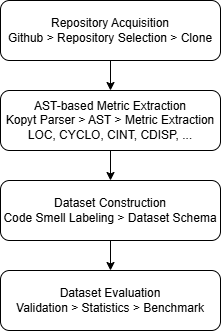
\includegraphics[width=0.3\linewidth]{fig/Metodology-Diagram}
	\caption{Dataset Construction Methodology}
	\label{fig:pic_studymethodology}
\end{figure}

\subsection{Repository Selection}

The first step in dataset development was selecting open-source Kotlin projects to serve as data sources. GitHub was selected for this repository, as it offers a diverse range of projects with varying characteristics and open documentation and development history. To ensure the quality and representativeness of the dataset, each repository was selected based on a series of inclusion and exclusion criteria, such as Kotlin language dominance, active project status, and source code completeness. This selection process aims to obtain a collection of projects that reflect real-world software development practices, ensuring that the extracted software metrics can represent the characteristics of Kotlin applications in general.

\subsection{Data Collection}

Once a repository is selected, all source code is collected and processed through the dataset development pipeline. The process begins with cloning the repository, followed by parsing Kotlin files using the Kopyt library to create an Abstract Syntax Tree (AST). The AST structure is then used as the basis for extracting software metrics for each analyzed code entity. Next, each entity is assigned a code smell label based on the detection rules used before all information is compiled into a final dataset. This dataset development pipeline is designed to be automated so that the extraction process can be carried out consistently across all analyzed repositories.

\subsection{Metric Extraction}

Software metrics extraction is a key step in this research because it determines the quality of the resulting dataset. Unlike approaches that rely on regular expressions or text pattern matching, this research uses an Abstract Syntax Tree (AST)-based approach through the Kopyt library to obtain a structural representation of Kotlin source code. All software metrics are calculated through an AST traversal process, thus recognizing various Kotlin syntax constructs more accurately and reducing errors due to code variations. This pipeline is used to calculate various classic software metrics, including complexity, size, cohesion, and coupling metrics. In addition to explaining the definition of each metric, this subsection also outlines the implementation mechanism of the extraction algorithm used so that the calculation process can be reproduced in future research.

\subsubsection{AST Generation Using Kopyt}
The first step in the software metrics extraction process is to build a structural representation of the source code using an Abstract Syntax Tree (AST). This research utilizes Kopyt, a Python-based Kotlin parser capable of generating ASTs in accordance with Kotlin grammar. Each source file is parsed into a tree structure that represents syntactic elements, such as class declarations, functions, properties, expressions, and control structures. AST representation allows the analysis process to be based on program structure, rather than simply matching text patterns, resulting in more accurate and consistent information. Furthermore, using Kopyt allows the extraction pipeline to be run automatically without relying on the Android development environment or the project's compilation process.

\subsubsection{Software Metrics Extraction}

Once the AST is successfully created, the next step is to extract software metrics from each analyzed code entity. The extraction pipeline is designed to calculate various classic software metrics commonly used in code smell detection research, including size metrics, complexity metrics, coupling, cohesion, inheritance, and response metrics. All metrics are calculated through an AST traversal of relevant nodes, enabling comprehensive recognition of Kotlin's syntax characteristics. This approach avoids various limitations of regular expression-based methods, such as misidentification due to variations in writing format or the use of more complex Kotlin syntax features.

\subsubsection{Implementation of Metric Extraction Algorithms}

Each software metric is implemented as an extraction module that operates independently on the AST structure. The extraction algorithm utilizes a traversal process through specific nodes according to the definition of each metric. For example, the size metric is calculated based on the number of relevant declarations and lines of code, while the complexity metric is obtained by identifying branching and looping structures in the AST. The coupling metric is analyzed by tracing relationships between classes through object declarations, inheritance, interface implementations, and method calls. This modular approach allows each algorithm to be validated separately and simplifies the addition of new software metrics without changing the entire extraction pipeline.

\subsubsection{Pipeline Reproducibility}

One of the main goals of this research is to produce a software metrics extraction pipeline that can be reproduced by other researchers. The entire process, from source code parsing and AST generation to software metrics extraction and dataset construction, is implemented in a deterministic pipeline. By using the same configuration, parser, and extraction algorithm, the pipeline will produce consistent software metrics values ​​for identical source code. Furthermore, comprehensive documentation regarding the extraction stages, metric definitions, and dataset structure is provided so that other researchers can replicate the dataset construction process or develop the pipeline for different metrics or code smells.

\subsection{Code Smell Labeling}

After all software metrics have been successfully extracted, each code entity is assigned a code smell label to form a classification dataset. The labeling process is performed using predefined detection rules based on the characteristics of each code smell type. The labeling results are then verified to ensure consistency between the obtained software metrics values ​​and the resulting code smell categories. This stage aims to produce accurate labels so that the dataset can be used reliably in the development and evaluation of machine learning models.

\subsection{Dataset Schema}

The final stage is organizing the dataset into an organized and user-friendly structure. The dataset contains project identity attributes, information about the classes or methods analyzed, all extracted software metrics, and code smell labels that are the target classification targets. Each attribute is documented along with its data type to facilitate interpretation and use of the dataset by other researchers. With a well-structured and documented schema, the dataset is not only ready for use in machine learning experiments but also supports reproducibility and further research development.

\section{Results}\label{sec:Results}

\subsection{Metric Verification}

The primary objective of the proposed AST-based extraction pipeline is to accurately extract software metrics that represent the structural characteristics of Kotlin source code. Before the constructed dataset can be considered reliable for machine learning-based code smell detection, the correctness of the extracted metrics must be systematically verified. Since the proposed dataset contains both method-level and class-level metrics with varying computational complexity, this study adopts two complementary verification strategies.

\subsubsection{Verification Strategy}

Two complementary verification strategies were employed according to the characteristics of each software metric.

First, metrics whose values can be directly derived from Kotlin source code were verified through manual source code inspection. These metrics mainly describe software size, complexity, and method characteristics, including Lines of Code (LOC), Cyclomatic Complexity (CYCLO), Maximum Nesting Level (MAXNESTING), Number of Local Variables (NOLV), Number of Parameters (NOP), Number of Accessed Variables (NOAV), Number of Method Calls (NMCS), and Fan-Out (FANOUT). Their values were independently recalculated based on their formal definitions and compared with those produced by the proposed extraction pipeline.

Second, metrics requiring inter-method or inter-class analysis were verified using an independent AST-based implementation provided by the Detekt static analysis framework \cite{WibowoICITDA2025}. Unlike the proposed pipeline, which is implemented using Kopyt, Detekt independently constructs and traverses Kotlin Abstract Syntax Trees. Therefore, comparing the outputs generated by the two independent AST implementations provides stronger evidence of correctness than relying solely on manual calculations. This strategy is particularly suitable for metrics involving cohesion, coupling, and structural relationships whose manual calculation would be impractical across numerous instances.

To evaluate the proposed extraction pipeline, one hundred methods were selected using stratified random sampling from the final labeled dataset while preserving the original repository, package, class, and method identifiers. The selected instances represent multiple Kotlin projects, various software complexities, and both smell and non-smell samples. Each selected instance was verified using the most appropriate verification strategy according to the metric characteristics, and the agreement between the verification results and the values generated by the proposed Kopyt-based extraction pipeline was subsequently calculated.

\subsubsection{Selection of Representative Metrics}

Although the proposed dataset contains a comprehensive collection of software metrics, verifying every extracted metric individually would be impractical. Therefore, this study adopts a representative metric verification strategy based on the feature selection results obtained from our previous studies on Long Method and Feature Envy detection \cite{Wibowo2026}.

Previous studies identified twelve representative software metrics for Long Method detection and another twelve representative metrics for Feature Envy detection. These metrics consistently demonstrated the highest contribution to machine learning classification performance and therefore represent the most informative software characteristics for the two code smell types.

Despite targeting different code smells, several representative metrics are shared by both detection models because they describe fundamental structural properties of software. Specifically, LOC, CYCLO, MAXNESTING, TCC, and AMWNAMM were identified as dominant predictors for both Long Method and Feature Envy. Since these metrics have identical formal definitions regardless of the target code smell, verifying them separately would introduce unnecessary duplication without providing additional evidence regarding the correctness of the extraction pipeline.

After removing duplicated metrics, the verification process focuses on nineteen unique representative metrics covering software size, complexity, cohesion, coupling, method interaction, method characteristics, and class design. Verifying this representative metric set provides confidence that the proposed AST-based extraction pipeline accurately extracts the software characteristics required for multiple machine learning-based code smell detection tasks.

\begin{table}[htbp]
	\centering
	\caption{Distribution of Representative Metrics Across Code Smells}
	\label{tab:metrics_distribution}
	\vspace{0.2cm}
	
	\begin{tabularx}{\textwidth}{>{\hsize=1.6\hsize\raggedright\arraybackslash}X >{\hsize=0.4\hsize\raggedleft\arraybackslash}X}
		\toprule
		\textbf{Source} & \textbf{Number of Metrics} \\
		\midrule
		Long Method representative metrics & 12 \\
		Feature Envy representative metrics & 12 \\
		\midrule
		Shared metrics & 5 \\
		Unique representative metrics & 19 \\
		\bottomrule
	\end{tabularx}
\end{table}

Table \ref{tab:metrics_distribution} summarizes the relationship between the representative metrics identified for Long Method and Feature Envy. Although twenty-four representative metrics were obtained from the two previous studies, five metrics overlap because they characterize fundamental software properties that are equally important for both code smell types. Consequently, only nineteen unique metrics were verified in this study. This strategy eliminates redundant verification while ensuring that every distinct software characteristic contributing to code smell detection is validated.

\subsubsection{Verification Results}

Based on the representative metric set described previously, each unique metric was verified using the verification strategy most appropriate to its computational characteristics. Table~\ref{tab:metrics_verification_methods} summarizes the software quality category of each representative metric together with the verification approach adopted in this study.

As shown in Table \ref{tab:metrics_verification_methods}, eight representative metrics describing software size, complexity, and method characteristics were verified through manual source code inspection, whereas the remaining eleven metrics involving cohesion, coupling, and structural relationships were verified using the independent AST-based implementation provided by Detekt. This combination enables both directly observable source-code properties and structurally complex software characteristics to be validated using the most appropriate verification technique.

The verification results demonstrate a consistently high level of agreement between the proposed Kopyt-based extraction pipeline and the corresponding verification methods. Metrics verified manually showed complete consistency with their formal definitions, while metrics verified through the independent AST implementation also exhibited a very high level of agreement. These findings indicate that the proposed extraction pipeline accurately captures both method-level and class-level software characteristics required for constructing machine learning datasets for multiple code smell detection tasks.

\begin{table}[H]
	\centering
	\small
	\caption{Specification of Metrics, Categories, and Verification Methods}
	\label{tab:metrics_verification_methods}
	\vspace{0.2cm}
	
	\let\oldunderscore\_
	\renewcommand{\_}{\oldunderscore\allowbreak}
	
	\begin{tabularx}{\textwidth}{
			>{\hsize=1.5\hsize\raggedright\arraybackslash}X 
			>{\hsize=1.1\hsize\raggedright\arraybackslash}X 
			>{\hsize=0.6\hsize\centering\arraybackslash}X 
			>{\hsize=1.2\hsize\raggedright\arraybackslash}X 
			>{\hsize=0.6\hsize\centering\arraybackslash}X
		}
		\toprule
		\textbf{Metric} & \textbf{Category} & \textbf{Used in} & \textbf{Verification Method} & \textbf{Agreement} \\
		\midrule
		LOC & Size & LM, FE & Manual Inspection & \\
		CYCLO & Complexity & LM, FE & Manual Inspection & \\
		MAXNESTING & Complexity & LM, FE & Manual Inspection & \\
		NOLV & Method & LM & Manual Inspection & \\
		NOP & Method & FE & Manual Inspection & \\
		NOAV & Method & FE & Manual Inspection & \\
		NMCS & Method Interaction & LM & Manual Inspection & \\
		FANOUT & Coupling & FE & Manual Inspection & \\
		\midrule
		number\_constructor\_Not\allowbreak Default\allowbreak Constructor\_methods & Design & LM & Detekt AST & \\
		number\_final\_not\_static\_methods & Design & LM & Detekt AST & \\
		WOC & Design & LM & Detekt AST & \\
		TCC & Cohesion & LM, FE & Detekt AST & \\
		AMWNAMM & Class Metric & LM, FE & Detekt AST & \\
		CC & Complexity & LM & Detekt AST & \\
		LAA & Cohesion & LM & Detekt AST & \\
		CM & Method & FE & Detekt AST & \\
		FDP & Coupling & FE & Detekt AST & \\
		ATFD & Coupling & FE & Detekt AST & \\
		CFNAMM & Design & FE & Detekt AST & \\
		\bottomrule
	\end{tabularx}
\end{table}

Table \ref{tab:unique_verification_summary} summarizes the overall verification statistics obtained from one hundred representative instances and nineteen unique software metrics. Overall agreement is calculated as the percentage of matching metric values between the proposed Kopyt-based extraction pipeline and the corresponding verification method across all evaluated metric instances.

\begin{table}[H]
	\centering
	\caption{Overall Summary of Metric Verification}
	\label{tab:unique_verification_summary}
	\vspace{0.2cm}
	
	\begin{tabularx}{\textwidth}{
			>{\hsize=1.6\hsize\raggedright\arraybackslash}X
			>{\hsize=0.4\hsize\raggedleft\arraybackslash}X}
		\toprule
		\textbf{Verification Item} & \textbf{Value}\\
		\midrule
		Verified repositories & ...\\
		Verified instances & 100\\
		Representative metrics & 19\\
		Verification methods & 2\\
		Total verified metric values & ...\\
		Matching values & ...\\
		\midrule
		\textbf{Overall Agreement} & \textbf{... \%}\\
		\bottomrule
	\end{tabularx}
\end{table}

\section{Discussion}\label{sec:Discussion}

Discussion \dots


\section{Conclusions}\label{sec:Conclusions}

Conclusions \dots


\subsection*{Acknowledgment}

\Funding{Founding sources }

\Data{\NA}

\CompetingInterests{Completing interests}

\Credits{
Author 1: Data curation, \dots .
Author 2: Conceptualization, \dots
% See https://credit.niso.org/
}

%% Uncomment if you use two separate bibliography files.
%\setbiblabelwidth{1000}
\bibliographystyle{IEEEtran_for_EI} 
\bibliography{eisej_paper}

%% Uncomment if you use two separate bibliography files.
%\setbiblabelwidth{1000}
%\bibliographystyleS{IEEEtran_for_EI}
%\bibliographyS{S}


\appendix
\makeatletter
\def\mw@seccntformat#1{Appendix\ #1.\enspace}
\makeatother

\section{Exemplary appendix}\label{sec:A}

Appendix content. 

\end{document}
